\documentclass[border=10pt]{standalone}
\usepackage{tikz}\usepackage{amsmath}\usetikzlibrary{calc,arrows.meta}
\begin{document}
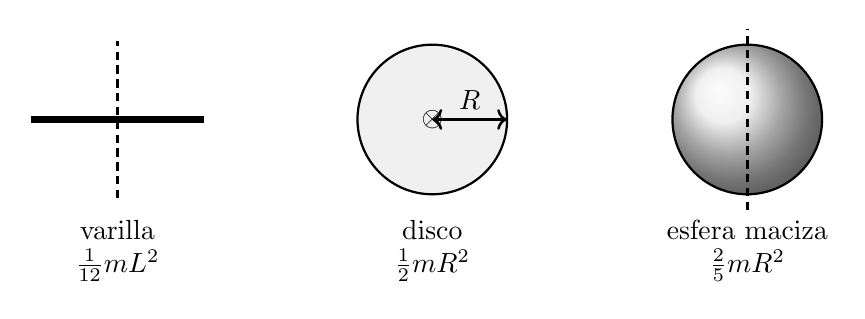
\begin{tikzpicture}[line width=0.9pt]
  % varilla
  \draw[densely dashed] (0,-1.0)--(0,1.0);
  \draw[line width=2.2pt] (-1.1,0)--(1.1,0);
  \node at (0,-1.4){varilla};
  \node at (0,-1.85){$\tfrac{1}{12}mL^2$};
  % disco
  \begin{scope}[xshift=4cm]
    \draw[thick,fill=black!6] (0,0) circle(0.95);
    \node at (0,0){$\otimes$};
    \draw[<->] (0,0)--(0.95,0) node[midway,above]{$R$};
    \node at (0,-1.4){disco};
    \node at (0,-1.85){$\tfrac12 mR^2$};
  \end{scope}
  % esfera
  \begin{scope}[xshift=8cm]
    \shade[ball color=black!8] (0,0) circle(0.95);
    \draw[thick] (0,0) circle(0.95);
    \draw[densely dashed] (0,-1.15)--(0,1.15);
    \node at (0,-1.4){esfera maciza};
    \node at (0,-1.85){$\tfrac25 mR^2$};
  \end{scope}
\end{tikzpicture}
\end{document}
